Wat waarschijnlijk wat uitleg behoeft is dat je prompt laat zien dat je je in de directory \~{} bevindt. Dat is geen
werkelijk bestaande directory maar een handige afkorting die we binnen de CLI kunnen gebruiken om de home-directory van
een gebruiker aan te duiden. Je eigen plek waar je je bestanden kan opslaan heet je home-directory en die kan dus ook
aangeduid worden met de \~{} (tilde). Je bevindt je dus in je eigen home-directory.

De werkelijke plek waar je je nu bevindt in het bestandssysteem kan je laten zien door
\begin{lstlisting}[language=bash]
$ pwd
\end{lstlisting}
te typen. Het pwd\index{pwd} commando toont de werk-directory en pwd staat dan ook voor print working directory. Je zult zien dat
pwd iets terug geeft als
\begin{lstlisting}[language=bash]
/home/dennis
\end{lstlisting}
waarbij `dennis' vervangen is door je eigen gebruikersnaam. De / (forward slash) is het scheidingsteken dat in Linux
gebruikt wordt om directory namen van elkaar te scheiden. Je bevindt je dus drie directories diep vanaf de root van het
bestandssysteem. / is de root-directory, home/ is de tweede directory en dennis/ is de derde directory.

Laten we eens kijken wat er in onze directory te vinden is. Om een overzicht te krijgen van de directories en bestanden
in onze directory typen we `ls'. `ls' is een afkorting voor list. Ofwel geef een lijst van aanwezige files en
directories. Afhankelijk van de distributie of de systeembeheerder zullen er al wat zaken aanwezig zijn. We gaan er
verder vanuit dat je een standaard CentOS installatie hebt gedaan zoals beschreven in een vorige hoofdstuk.

We gaan onze eerste eigen directory aanmaken. Type hiervoor:
\begin{lstlisting}[language=bash]
$ mkdir LinuxCursus
\end{lstlisting}
met behulp van `ls' kan je zien dat er een nieuwe directory bijgekomen is.

Met `cd', change directory, kunnen we ons verplaatsen in de directory:
\begin{lstlisting}[language=bash]
$ cd LinuxCursus
\end{lstlisting}
na de enter zal je zien dat de prompt gewijzigd is en een `ls' geeft een lege output omdat er
niets in de directory staat. Met `pwd' kan je controleren dat je daadwerkelijk in de nieuwe directory staat.

\begin{figure}
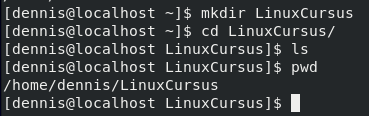
\includegraphics[width=3.8437in,height=1.2083in]{linuxreader-img027.png}
	\label{fig:CreateDirLinuxCursus}
	\caption{Het maken van de LinuxCursus directory}
\end{figure}

Nu gaan we een aantal directories tegelijk aanmaken hiervoor typen we:
\begin{lstlisting}[language=bash]
$ mkdir Data Documenten Muziek
\end{lstlisting}
na een `ls' zie je nu drie nieuwe directories. Zo zie je dat je door meerdere argumenten mee te
geven aan mkdir meer dan 1 directory kan aanmaken.

Met rmdir kan je directories weggooien.
\begin{lstlisting}[language=bash]
$ rmdir Data
\end{lstlisting}
Dit gooit de Data directory weg, na `ls' zie je nu nog maar twee directories.

Als we het systeem verder willen verkennen dan kunnen we met
\begin{lstlisting}[language=bash]
$ cd ~
\end{lstlisting}
ervoor zorgen dat we weer in onze home-directory terecht komen, dat scheelt toch een hoop typen die \~{}. \ Als we nu
\begin{lstlisting}[language=bash]
$ cd ..
\end{lstlisting}
typen dan gaan we terug in de directory boom. We komen in de /home/ directory terecht. De dubbele punten naast elkaar
(..) staan voor de directory die 1 stap lager ligt in de boom. We staan nu in de home/ directory die standaard alle
directories van alle gebruikers bevat, dus als er meer gebruikers op het systeem zouden zijn aangemaakt dan zouden ook
van deze gebruikers de home-directories hier te vinden zijn. Een uitzondering is de home-directory van de
systemadministrator van een Linux systeem. Deze beheerder heet `root' en zijn of haar directory is /root/. Daar komen
we later nog een keer op terug.

Als we weer
\begin{lstlisting}[language=bash]
$ cd ..
\end{lstlisting}
typen dan komen we in de / directory terecht. Lager kunnen we niet gaat op een Linux systeem, we zijn nu bij de
root-directory aangekomen. Let op de verwarring die kan ontstaan tussen de /root/ directory en de / directory beiden
heten de root-directory maar de ene is van de gebruiker root en de ander is van het bestandssysteem.

Met alleen het `cd' commando
\begin{lstlisting}[language=bash]
$ cd
\end{lstlisting}
kom je ook weer terug in je eigen home-directory.
